\documentclass{article}
\usepackage[slovak]{babel}
\usepackage[utf8]{inputenc}
\usepackage{hyperref}
\hypersetup{colorlinks=true, linkcolor=black, urlcolor=blue}
\usepackage{indentfirst}
\usepackage[left=2.5cm,text={16cm, 22cm},top=3.5cm]{geometry}
\usepackage{graphicx}

\begin{document}
    \begin{titlepage}
        \begin{center}
            \textsc{\Huge Vysoké učení technické v~Brně\\
            		\huge Fakulta informačních technologií\\}
            \vspace{\stretch{0.382}}
            {\LARGE IMP - Mikroprocesorové a vestavěné systémy\\}\vspace{2em}
            {\Large dokumentácia k projektu\\}\vspace{2em}
            \huge ARM-FITkit3: Hodiny s budíkem na bázi modulu Real Time Clock (RTC)\\
            \vspace{\stretch{0.618}}
        \end{center}
        {\Large \today \hfill Tomáš Nereča}\vspace{-2em}
    \end{titlepage}

    \tableofcontents
        \thispagestyle{empty}
        \newpage
        \setcounter{page}{1}
    \newpage
    
    \section{Úvod}
        Zadaním projektu bolo vytvoriť vstavanú aplikáciu \textbf{Digitálne hodiny s budíkom}.
        Aplikácia umožňuje:\\
        \begin{itemize}
            \item Nastaviť čas pre hodiny a budík
            \item Zapnúť/vypnúť funkciu budenia
            \item Zvoliť zvukovú a svetelnú signalizáciu
            \item Nastaviť opakovanie funkcie budenia
        \end{itemize}
        Aplikácia beží na platforme \textbf{FITKit 3} a využíva modul \textbf{RTC}.
        Je napísaná v jazyku C v prostredí \textbf{Kinetis Design Studio (KDS)}.
        Komunikácia s užívateľom prebieha cez rozhranie \textbf{UART}.
    
    \section{Implementácia}
        \subsection{Inicializácia a nastavenie parametrov}
        Po spustení aplikácie sú volané funkcie pre inicializáciu mikrokontroléru \textbf{MCU}, portov, rozhrania \textbf{UART} a modulu \textbf{RTC}.

        Následne je volaná funkcia \textbf{AppInit()}. V tejto funkcie sa na základe vstupu od užívateľa nastaví aktuálny čas a čas budenia.
        Užívateľ musí zadať čas vždy vo formáte HH:mm:ss. Vstup spracováva funkcia \textbf{GetTime()}, ktorá sa stará aj o prevod na sekundy.

        Po zadaní aktuálneho času sa spúšťa počítadlo času (register \textbf{TSR} modulu \textbf{RTC}).

        Po zadaní počtu opakovaní sa zadáva rozostup medzi opakovaniami, ak počet opakovaní nie je 0. Na záver je nastavený typ zvukovej a svetelnej signalizácie
        a do registru \textbf{TAR} priradený čas budenia. Všetky potrebné hodnoty su uložené v globálnych premenných, aplikácia beží v nekonečnom while cykle.

        \subsection{Ovládanie tlačidlami}
        \textbf{PORTE\_IRQHandler()} reaguje na stisk tlačidla. V podmienkach sa vyhodnotí, ktoré tlačidlo bolo stisknuté a na základe toho prebehne určitá operácia.
        Ide o zapnutie/vypnutie budenia (nastavuje sa globálny flag), zobrazenie aktuálneho času (hodnota z registru \textbf{TSR} sa prevedie na tvar HH:mm:ss
        funkciou \textbf{ConvertTime()}) a spustenie novej inicializácie (znovu je zavolaná funkcia \textbf{AppInit()}).

        \subsection{Prerušenie modulom RTC - budenie}
        \textbf{RTC\_IRQHandler()} je zavolaný, keď nastane čas budenia. V globálnej premennej \textbf{remainingRepeat} je počet pokusov o budenie, ktoré je treba vykonať.
        Ak je počet vačší ako 0, v registri \textbf{TAR} sa hodnota zvýši o rozostup medzi opakovaniami a počet zostávajúcich pokusov sa dekrementuje.
        Ak je počet rovný 0, v registri \textbf{TAR} sa hodnota nastaví na ďalší deň a počet zostávajúcich pokusov sa resetuje na počiatočnú hodnotu.

        Okrem toho sa spustí samotné budenie ak je v globálne premennej \textbf{alarmOn} hodnota 1. Funkcia \textbf{TurnOnLights()} spustí sveteľnú signalizáciu a funkcia \textbf{PlayMelody()} zvukovú.
        Zapínanie diód, delay a funkcia \textbf{Beep()} na vydanie tónu sú inšpirované laboratórnymi cvičeniami, podobne ako funkcie na inicializáciu, kde som čerpal aj z príkladov k FITkitu 3.

        \newpage

    \section{Použitie aplikácie}
        \subsection{Spustenie aplikácie}
            Po preložení a nahraní aplikácie do mikrokontroléru pomocou \textbf{KDS} je aplikácia pripravená na použitie a čaká na zadanie vstupných údajov.
            Komunikovať sa dá napríklad pomocou aplikácie \textbf{Putty} pod systémom \textbf{Windows}.
            Je potrebné otvoriť sériovú komunikáciu na porte \textbf{COMx} s parametrami:
            \begin{itemize}
                \item \textbf{Speed} - 115200
                \item \textbf{Data bits} - 8
                \item \textbf{Stop bits} - 1
                \item \textbf{Parity} - none
                \item \textbf{Flow control} - none
            \end{itemize}

        \subsection{Nastavenie parametrov}
            Aplikácia si postupne vyžiada zadanie nasledujúcich údajov:
            \begin{itemize}
                \item \textbf{Čas hodín} - Čas pre hodiny vo formáte HH:mm:ss (po zadaní sa hodiny spustia a čas beží!!!)
                \item \textbf{Čas budenia} - Čas budenia vo formáte HH:mm:ss (ak je čas menší ako čas pre hodiny, budenie prebehne až ďalší deň)
                \item \textbf{Počet opakovaní} - Číslo v rozmedzí 0-30, ide o počet opakovaných pokusov o budenie (potvrdiť stisknutím inej klávesy ako číslica, default hodnota je 0)
                \item \textbf{Interval medzi opakovaniami} - Číslo v rozmedzí 15-3600, ide o čas v sekundách medzi opakovanými pokusmi o budenie (potvrdiť stisknutím inej klávesy ako číslica, default hodnota je 60)
                \item \textbf{Zvuková notifikácia} - Číslo v rozmedzí 1-3, ide o melódiu zvukovej notifikácie 
                \item \textbf{Svetelná notifikácia} - Číslo v rozmedzí 1-3, ide o typ svetelnej notifikácie
            \end{itemize}
            Aplikácia teraz beží a v daný čas sa zapne funkcia budenia - najprv sa spustí svetelná notifikácia a následne zvuková.
            Pokiaľ by aplikácia bežala dosť dlho, budenie sa v ronaký čas zopakuje aj nasledujúci deň.

        \subsection{Funkcie tlačidiel}
            Aplikácia sa dá ovládať nasledujúcimi tlačidlami, ak je v stave po nastavení parametrov (aplikácia beží):
            \begin{itemize}
                \item \textbf{SW2} - Vypnutie/zapnutie funkcie budenia (aplikácia vypíše, v akom stave sa po prepnutí nachádza)
                \item \textbf{SW3} - Zobrazenie aktuálneho času vo formáte HH:mm:ss
                \item \textbf{SW4} - Nastavenie nových parametrov (rovnakým spôsobom ako po zapnutí aplikácie)
            \end{itemize}

        \subsection{Príklad spustenia}
            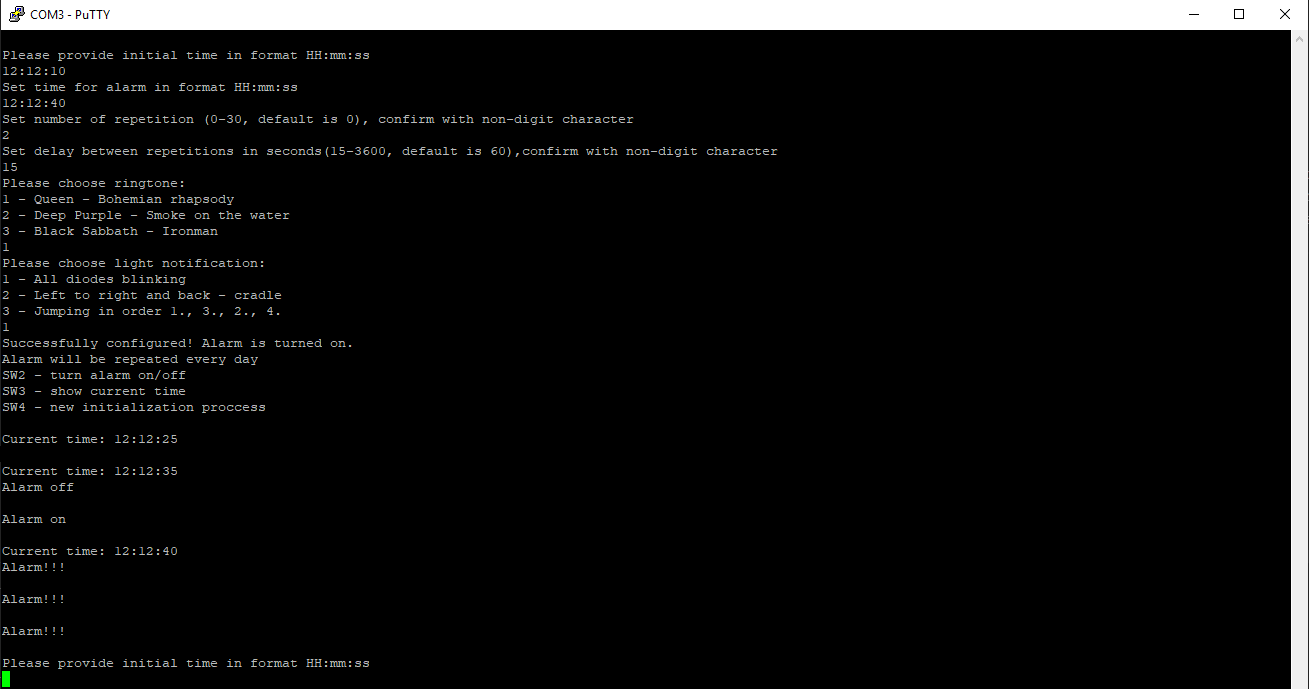
\includegraphics[width=15cm]{example.png}\\
            V tomto prípade je aplikácia spustená s budením o pár sekúnd od spustenia. Počet opakovaných pokusov o budenie je 2 s 15 sekundovými rozostupmi.
            Zvolená melódia je Bohemian Rhapsody a typ svetelnej notifikácie, kde blikajú všetky diódy naraz. Po nastavení parametrov je vypísaná nápoveda,
            aktuálny čas a čas budenia. O 10 sekúnd je stlačené tlačidlo pre vypísanie času, následne vypnutie a zapnutie budenia a potom samotné budenie, 2x opakované.
            Po budení je tlačidlom spustený proces nastavenia parametrov.
    
    \newpage
    
    \section{Literatúra}
    \noindent
    \url{https://wis.fit.vutbr.cz/FIT/st/cfs.php.cs?file=%2Fcourse%2FIMP-IT%2Fexcs%2FFITkit3-schema.pdf}\\
    \url{http://cache.freescale.com/files/32bit/doc/ref\_manual/K60P144M100SF2V2RM.pdf}\\
    \url{http://www.cplusplus.com/reference/}\\
    Študijné materiály k predmetu IMP - prednášky, laboratórne cvičenia, FITkit 3 examples\ldots\\
\end{document}